%%%%%%%%%%%%%%%%%%%%%%%%%%%%%%%%%%%%%%%%%%%%%%%%%%%%%%%%%%%%%%%%%%%%%%
% Lớp 12 | Ứng dụng đạo hàm để khảo sát hàm số | Cực trị của hàm số
% Dạng 2D1?2-3: Tìm 𝑚 để hàm số đạt cực trị tại 1 điểm 𝑥0 cho trước
% Số câu: 13  (sinh tự động bởi tach_cau.py; từ nay thầy sửa trực tiếp file này)
%%%%%%%%%%%%%%%%%%%%%%%%%%%%%%%%%%%%%%%%%%%%%%%%%%%%%%%%%%%%%%%%%%%%%%

%%%%%%%%%%%%%%%% TRẮC NGHIỆM 4 PHƯƠNG ÁN %%%%%%%%%%%%%%%%

% nguồn: Phan1_Lop_12_Dai_so_Chuong_1
\begin{ex}%[2D1H2-3]%[ma:d0a10a74]
	Cho hàm  số $y = 8x^3 -6mx^2 + 9mx + 6m$ ($m$ là tham số thực). Giá trị của $m$ để hàm số đạt cực tiểu tại $x=-6$ thuộc tập hợp nào sau đây?
	\choice 
		 {$\left(-\infty;-\dfrac{35}{3}\right)$}
		 {$\left(-\infty;-\dfrac{47}{3}\right)$}
		 {$\left(-\dfrac{23}{3}; +\infty\right)$}
		 {\True $\varnothing$}
	\loigiai{ 
		 Hàm số xác định với mọi $x \in \mathbb{R}$.\\
		Ta có $y'=24x^2 -12mx  + 9m$.\\
		Hàm số đạt cực tiểu tại $x=-6 \Rightarrow y'(-6) = 0 \Leftrightarrow 81m+864 = 0 \Leftrightarrow m=-\dfrac{32}{3}$.\\ 
		Với $m= -\dfrac{32}{3}$, ta được hàm số $y  = 8x^3 +64x^2 -96x -64$.\\
		Ta có $y'=24x^2 + 128x  -96$, $y'=0\Leftrightarrow 24x^2 + 128x -96=0\Leftrightarrow \hoac{&x=\dfrac{2}{3}\\&x=-6.}$\\
		Bảng biến  thiên
		\begin{center}
			\begin{tikzpicture}
				 \tkzTabInit[nocadre=false,lgt=1.2,espcl=2.5,deltacl=0.6]
					{$x$  /0.8,$y'$ /0.8,$y$ /2.5}
					 {$-\infty$,$-6$,$\tfrac{2}{3}$,$+\infty$}
				\tkzTabLine{,+,$0$,-,$0$,+,} 
				\tkzTabVar{-/$-\infty$,+/$1\,088$,-/$\dfrac{704}{27}$,+/$+\infty$} 
			\end{tikzpicture}
		\end{center}
		Suy ra hàm số đã  cho đạt cực đại tại điểm $x=-6$ và đạt cực tiểu tại điểm $x=\dfrac{2}{3}$.\\
		Vậy không có giá trị nào của $m$ thoả  bài toán.
	} 
\end{ex}

% nguồn: Phan1_Lop_12_Dai_so_Chuong_1
\begin{ex}%[2D1V2-3]%[ma:6a451331]
	Tìm $m$ để hàm số $y = x^3 - 3mx^2 + (m^2 + 2)x - m + 1$ đạt cực đại tại $x = 1$. 
	\choice 
		{$\hoac{&m = 1\\&m  = 5}$.}
		 {Không tồn tại $m$}
		{$m  = 1$}
		{\True $m =  5$}
	\loigiai{ 
		Ta  có: $y'= 3x^2 - 6mx + (m^2 + 2), y''=6x -6m$.\\
		Hàm số $y = x^3 - 3mx^2 + (m^2 + 2)x - m + 1$ đạt cực đại tại $x = 1$ khi và chỉ  khi
		\begin{eqnarray*}
			& &\heva{&y'(1) =  0\\&y''(1) = 0}\\
			&\Leftrightarrow& \heva{&3 - 6m + m^2 +  2= 0\\&6 - 6m < 0}\\
			&\Leftrightarrow& \heva{&m^2 - 6m + 5 = 0\\&m >  1}\\
			 &\Leftrightarrow& \heva{&\hoac{&m = 1\\&m = 5}\\&m > 1}\\
			 &\Leftrightarrow& m = 5.
		\end{eqnarray*}
	 }
\end{ex}

% nguồn: Phan1_Lop_12_Dai_so_Chuong_1
\begin{ex}%[2D1V2-3]%[ma:a1b1db0f]
	Giá trị nguyên lớn nhất của tham số $m$ để hàm số $y = \dfrac{x^2 + (m  - 1)x + 3 - 2m}{x + m}$ đạt cực tiểu tại $x = -1$ thuộc khoảng nào sau đây?
	\choice 
		{\True $(0;\sqrt{5})$} 
		 {$(-2;0)$}
		 {$(-1;2)$}
		 {$(\sqrt{55};5)$}
	 \loigiai{
		Điều kiện xác định  $x \ne m$.\\
		Đạo hàm cấp một và cấp hai của hàm số lần lượt là: $y'= 1 + \dfrac{m - 3}{(x + m)^2}, y''=\dfrac{-2(m - 3)}{(x +  m)^3}$.\\
		Để hàm số đạt cực tiểu tại $x = -1$ khi và chỉ khi: $\heva{&y'(-1) = 0\\&y''(-1) > 0\\&m \ne 1} \Leftrightarrow \heva{&1 + \dfrac{m - 3}{(x  + m)^2}=0\\&\dfrac{-2(m - 3)}{(x + m)^3} > 0\\&m \ne 1} \Leftrightarrow \hoac{&m = 2\\&m = -1}$.\\
		Nghiệm nguyên lớn nhất của $m = 2$ nên chọn khoảng  $(0;\sqrt{5})$.
	} 
\end{ex}

% nguồn: Phan1_Lop_12_Dai_so_Chuong_1
\begin{ex}%[2D1V2-3]%[ma:6bd0672c]
	Tìm tất cả các giá trị của tham số $m$ để hàm số $y = x^3 - (2m  -1)x^2 - (5m + 4)x + 10$ đạt cực đại tại điểm $x = -1$.
	 \choice
		{$m =  -1$}
		{$m  = 3$}
		{\True $m = 1$} 
		{$m =- 2$} 
	 \loigiai{
		Ta có: $y' = 3x^2 - 2(2m - 1)x - (5m +  4)$ và $y''= 6x - 2(2m + 1)$\\
		Hàm số đạt cực đại tại điểm $x = -1$ khi $\heva{&y'(-1) = 0\\&y''(-1) < 0} \Leftrightarrow \heva{&-m + 1 = 0\\&-4m - 8< 0}  \Leftrightarrow \heva{&m=1\\&m > -2} \Rightarrow m = 1$.
	} 
\end{ex}

% nguồn: Phan1_Lop_12_Dai_so_Chuong_1
\begin{ex}%[2D1V2-3]%[ma:58d3fed7]
	Cho  hàm số $y = x^3 + 3(m^2 - m +2)x^2 + 3(3m^2 + 1)x + 2022m$, tìm các giá trị của tham số $m$ để hàm số đạt cực tiểu tại $x=-2.$
	\choice 
		{$m =  1$}
		{$m = 2$} 
		{\True  $m = 3$}
		 {$m=4$}
	\loigiai{ 
		Ta có: $y'=3x^2 + 6(m^2 - m + 2)x + 3(3m^2 + 1)=3[x^2 + 2(m^2 -  m + 2)x + 3m^2 + 1]$;\\
		$y''= 6x + 6(m^2 -  m + 2)$.\\
		Hàm  số đạt cực tiểu tại $x= -2$ khi và chỉ khi
		\begin{eqnarray*}
			& & \heva{&y'(2) = 0\\&y''(2)  > 0} \\
			&\Leftrightarrow& \heva{&m^2 - 4m + 3 =0\\&6m(m-1) > 0}\\ 
			&\Leftrightarrow& \heva{&\hoac{&m=1\\&m=3}\\&m(m - 1) >  0}\\
			&\Leftrightarrow& m  = 3.
		\end{eqnarray*}
	 }
\end{ex}

% nguồn: Phan1_Lop_12_Dai_so_Chuong_1
\begin{ex}%[2D1V2-3]%[ma:210ac071]
	Tìm giá  trị thực của tham số $m$ để hàm số $y = \dfrac{1}{3}x^3 - mx^2 + (m^2 - m - 1)x$ đạt giá trị cực đại tại $x = 1$.
	 \choice
		{$m =  2$}
		{$m = 1$} 
		{\True $m  = 3$}
		{$m = 0$} 
	 \loigiai{
		Tập xác định $D  = \mathbb{R}$.\\
		Ta có: $y' = x^2 - 2mx + m^2 - m  -1$ và $y''=2x - 2m$.\\
		Hàm số đạt cực đại tại $x = 1$ nên $y'(1)= 0 \Leftrightarrow m^2  - 3m = 0 \Leftrightarrow \hoac{&m = 0\\&m = 3.}$\\
		Với $m = 0$ thì $y''(1) = 2 > 0$  suy ra hàm đạt cực tiểu tại $x =1$ (loại).\\
		Với $m = 3$ thì $y''(1) =  -4 < 0$ suy ra hàm đạt cực đại tại $x =1$ (nhận).\\
		 Vậy $m = 3$ là giá trị cần tìm.
	 }
\end{ex}

% nguồn: Phan1_Lop_12_Dai_so_Chuong_1
\begin{ex}%[2D1V2-3]%[ma:022ed64d]
	Cho hàm số $f(x) = -x^3 + 2(2m - 1)x^2 - (m^2 - 8)x + 2$.  Tìm tất cả các giá trị của tham số $m$ để hàm số đạt giá trị cực địa tại điểm $ x = -1$.
	 \choice
		{$m  = 3$}
		{\True  $m = -9$}
		{$m =  1$}
		{$m = -2$} 
	 \loigiai{
		Ta có $f'(x)=-3x^2 + 4(2m -1)x  - (m^2 - 8)$\\
		Hàm số  đtaj giá trị cực đại tại điểm $x = -1 \Rightarrow f'(-1) = 0 \Rightarrow -m^2 - 8m + 9 = 0 \Leftrightarrow \hoac{&m = 1\\&m = -9}$\\
		Với  $m =1 \Rightarrow f(x) = -x^3 + 2x^2 + 7x + 2$\\
		Có $f'(x) = -3x^2 + 4x + 7;  f''(x) = -6x + 4$\\
		Mà $\heva{&f'(-1) = 0\\&f''(-1) = 10 > 0} \Rightarrow$ Hàm  số đạt cực tiểu tại $x = -1 \Rightarrow m = 1$ không thỏa mãn yêu cầu bài toán.\\
		 Với $m = -9 \Rightarrow f(x) = -x^3 - 38x^2 - 73x + 2$\\
		Ta có: $f'(x) = -3x^2 - 76x -73; f''(x)  = -6x - 76$\\
		Mà $\heva{&f'(-1) =  0\\&f''(-1) = -70 < 0} \Rightarrow$ Hàm số đạt cực đại tại $x = -1 \Rightarrow m = -9$ thỏa mãn yêu cầu bài toán.\\
		Vậy $m  = -9$ thỏa mãn đề bài.
	} 
\end{ex}

% nguồn: Phan1_Lop_12_Dai_so_Chuong_1
\begin{ex}%[2D1V2-3]%[ma:41dc566a]
	Tìm tất cả các giá trị của tham số  $m$ để hàm số $y= \dfrac{1}{3}x^3 + mx^2 + (m^2 - 2m - 3)x + 4$ đạt cực tiểu tại điểm $x = 0$.
	\choice 
		{$m = -1$  hoặc $m = 3$}
		{$m  = -1$}
		{\True $m = 3$} 
		{$m =  1$ hoặc $m = 3$}
	 \loigiai{
		Tập xác định: $D = \mathbb{R}$. Đạo hàm $y' = x^2 + 2mx + m^2 -  2m -3$.\\
		Hàm số $y= \dfrac{1}{3}x^3 +  mx^2 + (m^2 - 2m - 3)x + 4$ đạt cực tiểu tại điểm $x = 0$
		$\Rightarrow y'(0) = 0 \Leftrightarrow 0^2 + 2m \cdot 0 + m^2 - 2m -3  = 0 \Leftrightarrow m^2 - 2m - 3 = 0 \Leftrightarrow \hoac{&m = -1\\&m = 3}$.\\
		Với $m = -1, y'= x^2 - 2x, y'= 0 \Leftrightarrow \hoac{&x = 0\\&x = 2};  y''= 2x -2 \Rightarrow y''(0) = -2 < 0$\\
		Hàm số $y= \dfrac{1}{3}x^3 + mx^2 + (m^2 - 2m - 3)x + 4$  đạt cực đại tại điểm $x = 0$ khi $m = -1$.\\
		Vậy $m = -1$ không thỏa mãn yêu cầu bài toán.\\ 
		Với $m = 3, y' = x^2 + 6x, y'  = 0 \Leftrightarrow x^2 + 6x = 0 \Leftrightarrow \hoac{&x = 0\\& x= -6}; y''= 2x + 6 \Rightarrow y''(0)= 6 > 0$.\\
		Hàm số $y = \dfrac{1}{3}x^3 + mx^2 + (m^2 - 2m - 3)x + 4$ đạt  cực tiểu tại điểm $x = 0$ khi $m = 3$ (thỏa mãn).
	} 
\end{ex}

% nguồn: Phan1_Lop_12_Dai_so_Chuong_1
\begin{ex}%[2D1V2-3]%[ma:09948d17]
	Tìm tất cae các giá trị thực của tham số $m$ để hàm số $y=x^3 - 3x^2 + mx + 1$ đạt  cực tiểu tại $x=2$?
	 \choice
		{$0<m \leq  4$}
		 {$m > 4$}
		 {\True$m=0$}
		{$0 \leq m  < 4$}
	 \loigiai{
		Ta có: $y=x^3 - 3x^2 + mx  + 1$\\
		Khi đó $y'=3x^2 - 6x + m; y''=6x -  6$\\
		Hàm số đạt cực tiểu  tại $x=2 \Leftrightarrow
		\heva{&y'(2) =  0\\&y''(2) > 0} \Leftrightarrow
		\heva{&m = 0\\&6 > 0}\Leftrightarrow m =  0.$
	 }
\end{ex}

% nguồn: Phan1_Lop_12_Dai_so_Chuong_1
\begin{ex}%[2D1V2-3]%[ma:54bbda84]
	Gọi  $S$ là tập hợp tất cả các giá trị của tham số $m$ để hàm số $y= mx^3 - (m^2 + 1)x^2 + 2x - 3$ đạt cực tiểu tại $x=1$. Khi đó?
	 \choice
		 {$S=\left\{\dfrac{-3}{2}\right\}$}
		{$S  = \{0\}$}
		 {$S = \left\{\dfrac{3}{2}; 0\right\}$}
		{\True  $S=\left\{\dfrac{3}{2}\right\}$}
	\loigiai{ 
		\textbf{TH1:} $m = 0 \Rightarrow y = -x^2 + 2x - 3 \Rightarrow $ Hàm số  chỉ có cực đại.\\
		\textbf{TH2:} $m \ne 0 \Rightarrow \heva{&y' = 3mx^2 - 2(m^2 + 1)x  + 2\\&y''=6mx - 2(m^2 + 1)}$\\
		Do hàm số đã cho là hàm bậc 3 nên điều kiện cần để hàm đạt cực tiểu tại $x = 1$ là\\ 
		$y'(1) = 0 \Leftrightarrow 3m  - 2(m^2 + 1) + 2= 0 \Leftrightarrow \hoac{&m = 0\\&m = \dfrac{3}{2}} \Rightarrow m = \dfrac{3}{2}$\\
		Khi $m = \dfrac{3}{2}$ ta có $y''(1)= 9 - 2\left(\dfrac{9}{4} + 1\right) = \dfrac{5}{2} > 0$ nên $m = \dfrac{3}{2}$ thỏa mãn 
	} 
\end{ex}

% nguồn: Phan1_Lop_12_Dai_so_Chuong_1
\begin{ex}%[2D1V2-3]%[ma:a595d603]
	Khi hàm số $y = -\dfrac{1}{3}x^3 - mx^2  + (m^2 - 2)x + 2021$ đạt cực đại tại $x =1$ thì giá trị của tham số $m$ thuộc khoảng nào sau đây?
	 \choice
		{\True  $(1;4)$}
		{$(-3;0)$} 
		 {$(0;3)$}
		{$(-2;0)$} 
	\loigiai{ 
		Ta có: $y' = -x^2 - 2mx + m^2 -  2$ và $y''= -2x - 2m$.\\
		Hàm số đạt cực đại tại $x  =1$ thì
		\begin{eqnarray*}
			& & y'(1) =  0\\
			&\Leftrightarrow& -1^2 - 2m\cdot  1 + m^2 - 2 = 0\\
			&\Leftrightarrow& m^2 - 2m -  3 = 0\\
			&\Leftrightarrow& \hoac{&m  = 3\\&m = -1}.\\
		\end{eqnarray*}
		Với $m = 3$ ta có $y''(1) = -2\cdot 1 - 2\cdot 3= -8 < 0$  nên $x = 1$ là điểm cực đại.\\
		Suy ra  $m = 3$ thỏa mãn.\\
		Với $m = -1$ ta có $y'  = -x^2 + 2x - 1 = -(x - 1)^2 \le 0 \Rightarrow$ hàm số luôn nghịch biến, nên hàm số không có cực trị.\\
		Suy ra $m =  -1$ không thỏa mãn.\\
		Vậy $m = 3$ thì hàm số $y = -\dfrac{1}{3}x^3 - mx^2 +  (m^2 - 2)x + 2021$ đạt cực đại tại $x =1$.
	} 
\end{ex}

% nguồn: Phan1_Lop_12_Dai_so_Chuong_1
\begin{ex}%[2D1V2-3]%[ma:584fa3c7]
	Cho hàm số $y = x^3  + (m^2 - m + 1)x^2 + (3m^2 - 4)x + m + 2$. Có bao nhiêu giá trị của $m$ để hàm số đạt cực tiểu tại $x = -1$?
	\choice 
		 {$0$}
		{\True  $1$}
		{$2$} 
		{$3$} 
	 \loigiai{
		Ta có: $y' = 3x^2 + 2(m^2 -  m + 1)x + 3m^2 - 4$ và $y''= 6x + 2(m^2 - m + 1)$\\
		Hàm số đạt cực tiểu tại $x = -1$ thì $y'(-1) =  0 \Leftrightarrow m^2 + 2m - 3 = 0 \Leftrightarrow m = 1; m = -3$\\
		Thử lại:\\ 
		Khi $m  = 1$, $y''(-1) < 0$: Hàm số đạt cực đại tại $x = -1$ (Không thỏa yêu cầu bài toán)\\
		Khi $m = -3$, $y''(-1) > 0$: Hàm số đạt cực tiểu tại $x = -1$ (Thỏa yêu cầu bài  toán)\\
		Vậy có 1 giá  trị của $m$ thỏa mãn.
	 }
\end{ex}


%%%%%%%%%%%%%%%% TRẢ LỜI NGẮN %%%%%%%%%%%%%%%%

% nguồn: Phan2_Lop_12_Dai_so_Chuong_1
\begin{bt}%[2D1V2-3]%[ma:74145205]
	Hàm số $y = \dfrac{2}{3}x^3 - mx^2 - 2(3m^2 - 1)x + \dfrac{2}{3}$ có $2$ điểm cực trị $x_1,x_2$ sao cho $x_1x_2 + 2(x_1 + x_2) = 1$ khi $m  = \dfrac{a}{b}$. Tính $S= a^2 + b^2$.
	 \shortans{13}
	 \loigiai{
		Ta có: $y = \dfrac{2}{3}x^3 - mx^2 -  2(3m^2 - 1)x + \dfrac{2}{3} \Rightarrow y' = 2x^2 - 2mx - 2(3m^2 - 1)$.\\
		Để $y$ có hai cực trị $x_1,x_2$ thì phương trình $y' = 0$  có hai nghiệm phân biệt, tức là:\\
		$\Delta' = m^2 + 4(3m^2 - 1) = 13m^2 - 4 > 0$ hay $m \in  \left(-\infty; -\dfrac{2}{\sqrt{13}}\right) \cup \left(\dfrac{2}{\sqrt{13}};+\infty\right)$.\\
		Ta lại có $x_1x_2 + 2(x_1 + x_2) = 1 \Leftrightarrow -3m^2 + 1 + 2m = 1  \Leftrightarrow -3m^2 + 2m = 0$\\
		$\Leftrightarrow \hoac{&m = 0 \text{ (loại)}\\&m = \dfrac{2}{3} \text{ (thỏa)}} \Rightarrow \heva{&a = 2\\&b= 3} \Rightarrow  S=13$.
	} 
\end{bt}
